\newpage
\section{Восстановление объектных структур данных при декомпиляции при отсутствии информации о типах времени выполнения}\label{chapter:reconstruction_without_rtti}
В связи с тем, что использование информации о типах времени выполнения в программах на языке Си++ считается <<дурным тоном>>, и зачастую используется неправильно \cite{stroustrup93}, сегодня существуют программные продукты, не использующие информацию о типах времени выполнения. В случае, если программа была скомпилирована без информации о типах времени выполнения, для каждого полиморфного класса по-прежнему генерируется таблица виртуальных функций. Вообще говоря, уникальность таблицы для каждого класса не гарантируется, и компилятор может объединить таблицы для двух полиморфных классов \lstinline{Base} и \lstinline{Derived}, если \lstinline{Base} является предком \lstinline{Derived} и при этом \lstinline{Derived} не {\it перекрывает} ни одну из виртуальных функций, объявленных в \lstinline{Base}. Однако в случае, если хотя бы одна из добавленных в \lstinline{Derived} виртуальных функций не являются {\it чисто виртуальной}, компиляторы GCC и MSVC создают для \lstinline{Derived} отдельную таблицу виртуальных функций. 
%Таким образом, если найти все таблицы виртуальных функций, то путем анализа их структуры и входящих в них функций можно восстановить иерархию полиморфных классов программы.

Как было отмечено в главе \ref{chapter:problem}, для корректного восстановления иерархии классов некоторой ассемблерной программы $\bA$, полученной путем компиляции программы на языке Си++ $\bP$, необходимо построить множество классов $\gCa$, и восстановить отношение непосредственного наследования $\leftarrow \; \subseteq \gCa \times \gCa$. В дальнейшем будем рассматривать отношение\footnote{Здесь и далее определения используемых обозначений даны в приложении А.} $\lhd = \enspace \leftarrow^+$. $\lhd$ является отношением строгого частичного порядка, так как оно:
\begin{itemize}
\item Антирефлексивно: $\forall A \in \gCa: \neg (A \lhd A)$;
\item Ассиметрично: $\forall B, D \in \gCa: B \lhd D \Longrightarrow \neg (D \lhd B)$;
\item Транзитивно: $\forall B, C, D \in \gCa: B \lhd C \wedge C \lhd D \Longrightarrow B \lhd D$.
\end{itemize}

Это в частности означает, что отношение $\leftarrow$ восстанавливается по отношению $\lhd$ следующим образом: $\leftarrow \; = \lhd \setminus \lhd \circ \lhd$.

В дальнейшем будем предполагать, что компилятор, с помощью которого была скомпилирована исследуемая программа, известен. Информация о компиляторе могла быть получена как с использованием методов, описанных в главе \ref{chapter:rtti_extraction}, так и из внешних источников.

%Обозначим множество всех таблиц виртуальных функций программы $VTables$. Для удобства введем также отображение $ClassOf: VTables \rightarrow \gC$, возвращающее для каждой таблицы виртуальных функций соответствующий ей класс. Аналогично с введенным на множестве $\gC$ отношением $\leftarrow$, введем отношение $\leftarrow$ и на множестве $VTables$: будем говорить, что таблица виртуальных функций $d$ является непосредственным наследником таблицы виртуальных функций $b$, то есть $b \leftarrow d$, тогда и только тогда, когда $ClassOf(b) \leftarrow ClassOf(d)$.

%Аналогично с отношением $\lhd$ на множестве классов определим это отношение и на множестве таблиц виртуальных функций: $\lhd = \; \leftarrow^+$. Для отношения $\lhd$ на множестве таблиц виртуальных функций будем применять те же термины, что и для отношения $\lhd$ на множестве классов.


\subsection{Обработка множественного наследования}\label{chapter:multiple_inheritance}
Так как для классов, имеющих несколько непосредственных базовых полиморфных классов, компиляторы GCC и MSVC генерируют несколько таблиц виртуальных функций --- по одной таблице на каждую таблицу виртуальных функций каждого непосредственного базового полиморфного класса \cite{gray94, gccabi}, то в общем случае отличить множественное наследование от одиночного оказывается затруднительно. На рис. \ref{fig:multiple_base_example_vtable} представлены сгенерированные компилятором MSVC таблицы виртуальных функций для иерархии классов, представленной на рис. \ref{listing:multiple_base_example}.

\begin{figure}[htb!]
\hspace{2cm}
\begin{minipage}[b]{1cm}
\begin{cplusplus}
class A {
public:
    virtual void a() {/* ... */}
};

class B {
public:
    virtual void b() {/* ... */}
};

class C: public A, public B {
public:
    virtual void a() {/* ... */}
    virtual void b() {/* ... */}
};
\end{cplusplus}
\end{minipage}
\caption{Пример использования множественного наследования в Си++.}
\label{listing:multiple_base_example}
\end{figure}

\begin{figure}[htb!]
\hspace{2cm}
\begin{minipage}[b]{1cm}
\lstinline!const A::`vftable'! \\
\fbox{\lstinline{&A::a(void)}} \\
\\
\lstinline!const B::`vftable'! \\
\fbox{\lstinline{&B::b(void)}} \\
\\
\lstinline!const C::`vftable'{for `A'}! \\
\fbox{\lstinline{&C::a(void)}} \\
\\
\lstinline!const C::`vftable'{for `B'}! \\
\fbox{\lstinline{&C::b(void)}}
\end{minipage}
\caption{Таблицы виртуальных функций, сгенерированные компилятором MSVC для иерархии классов, представленной на рис. \ref{listing:multiple_base_example}.}
\label{fig:multiple_base_example_vtable}
\end{figure}

\begin{figure}[htb!]
\hspace{2cm}
\begin{minipage}[b]{1cm}
\begin{cplusplus}
class B1: public B {
public:
    virtual void b() {/* ... */}
};

class C: public A {
private:
    B1 b;
public:
    virtual void a() {/* ... */}
};
\end{cplusplus}
\end{minipage}
\caption{Модифицированная иерархия наследования.}
\label{listing:multiple_base_example_modified}
\end{figure}

Сравним приведенное на рис. \ref{listing:multiple_base_example_modified} альтернативное описание класса \lstinline{C} c приведенным на рис. \ref{listing:multiple_base_example}. Как видно, альтернативное описание было получено путем переноса метода \lstinline{C::b(void)} из класса \lstinline{C} в производный от \lstinline{B} класс \lstinline{B1}, удаления класса \lstinline{B} из списка базовых классов для класса \lstinline{C}, и добавления нового поля типа \lstinline{B1} в класс \lstinline{C}. При такой организации иерархии множественное наследование было заменено одиночным наследованием с добавлением поля. В результате проведения экспериментов было выяснено, что для иерархий, представленных на рис. \ref{listing:multiple_base_example} и рис. \ref{listing:multiple_base_example_modified}, компилятор MSVC генерирует таблицы виртуальных функций, имеющие одинаковую структуру --- такую же, как на рис. \ref{fig:multiple_base_example_vtable}. Дальнейшее исследование полученных в результате компиляции ассемблерных программ показало, что они эквивалентны в смысле, определенном в \cite{dolgova08}. Такие же результаты были получены и для компилятора GCC.

\begin{figure}[htb!]
\hspace{2cm}
\begin{minipage}[b]{1cm}
\begin{cplusplus}
class B1 {
    /* ... */
public:
    virtual b1() {/* ... */}
};

class B2 {
    /* ... */
public:
    virtual b2() {/* ... */}
};

class D: public B1, public B2 {
    /* ... */
public:
    virtual b2() {/* #\tl{обращение к полям B1}@ */}
};
\end{cplusplus}
\end{minipage}
\caption{Пример иерархии классов, в виртуальных функциях классов которой возможно обращение по отрицательному смещению относительно переданного в функцию указателя \lstinline{this}.}
\label{listing:negative_this_access}
\end{figure}

В некоторых случаях использование множественного наследования можно выявить. Один из таких случаев --- наличие обращения по отрицательному смещению относительно указателя \lstinline{this} в одной из виртуальных функций. Рассмотрим пример, приведенный на рис. \ref{listing:negative_this_access}. Согласно используемым в компиляторах GCC и MSVC бинарным интерфейсам приложений \cite{gray94, gccabi}, объект класса \lstinline{D} будет иметь структуру, представленную на рис. \ref{fig:class_layout}.

\begin{figure}[htb!]
\centering
\includegraphics[scale=1.0]{images/class_layout.png}
\caption{Структура объекта класса \lstinline{D}, описанного на рис. \ref{listing:negative_this_access}.}
\label{fig:class_layout}
\end{figure}

При вызове виртуальной функции \lstinline{D::b2} в качестве указателя \lstinline{this} ей будет передан не указатель на начало объекта класса \lstinline{D}, а указатель на начало экземпляра класса \lstinline{B2} внутри этого объекта. Функция \lstinline{D::b2} работает с полями, унаследованными классом \lstinline{D} от \lstinline{B1}, и так как экземпляр класса \lstinline{B1} предшествует экземпляру класса \lstinline{B2} внутри объекта класса \lstinline{D}, как это изображено на рис. \ref{fig:class_layout}, то обращение к этим полям будет производиться по отрицательному смещению относительно переданного в функцию \lstinline{D::b2} указателя \lstinline{this}. Заметим, что в случае одиночного наследования такая ситуация невозможна.

Еще один случай, в котором можно выявить множественное наследование, связан с использованием виртуальных деструкторов. Рассмотрим пример, приведенный на рис. \ref{listing:multiple_base_vdestructor}.

\begin{figure}[htb!]
\hspace{2cm}
\begin{minipage}[b]{1cm}
\begin{cplusplus}
class B1 {
public:
    virtual ~B1() {/* ... */}
};

class B2 {
public:
    virtual ~B2() {/* ... */}
};

class D: public B1, public B2 {
public:
    virtual ~D() {/* ... */}
};
\end{cplusplus}
\end{minipage}
\caption{Пример использования виртуальных деструкторов в иерархии с множественным наследованием.}
\label{listing:multiple_base_vdestructor}
\end{figure}

В данном примере для класса \lstinline{D} генерируется две таблицы виртуальных функций --- по одной для каждого полиморфного базового класса. При этом обе таблицы должны содержать указатель на виртуальный деструктор класса \lstinline{D}. Однако при вызове виртуального деструктора для класса \lstinline{B2}, ему передается указатель не на объект класса \lstinline{D}, а на экземпляр класса \lstinline{B2} внутри объекта класса \lstinline{D}. Поэтому в таблице виртуальных функций класса \lstinline{D}, соответствующей классу \lstinline{B2}, хранится указатель не на виртуальный деструктор класса \lstinline{D}, а на {\it адаптер}, производящий выравнивание переданного указателя \lstinline{this} таким образом, чтобы он указывал на начало объекта класса \lstinline{D}, и передающий управление виртуальному деструктору. Размер полиморфного класса всегда больше нуля, так как объекты такого класса хранят указатель на таблицу виртуальных функций, и поэтому различным полиморфным базовым классам с виртуальными деструкторами соответствуют различные адаптеры. По коду такого адаптера также можно определить смещение базового класса внутри объемлющего. Метод выявления виртуальных деструкторов описан в главе \ref{chapter:destructors}.

Так как большинство иерархий классов используют виртуальные деструкторы, то изложенные выше факты в большинстве случаев дают возможность выявить использование множественного наследования, и определить, какие таблицы виртуальных функций принадлежат одному и тому же классу. В случае отсутствия виртуальных деструкторов можно выявить факт использования множественного наследования, но определить, какие таблицы виртуальных функций принадлежат одному и тому же классу, оказывается затруднительно. Также не смотря на то, что обращение по отрицательному относительно указателя \lstinline{this} смещению подразумевает использование множественного наследования, такое обращение возможно и при использовании одиночного наследования при наложении дополнительных ограничений на параметры функции. В результате проведения экспериментов было выяснено, что в случае отсутствия виртуальных деструкторов, для программы на языке Си++ $\bP$, использующей множественное наследование, и соответствующей ей программы на языке ассемблера $\bA$, возможно построить программу $\bP'$, использующую лишь одиночное наследование, при компиляции которой получается ассемблерная программа $\bA'$, эквивалентная $\bA$. Метод построения такой программы основан на тех же приемах, что были приведены выше в комментариях к рис. \ref{listing:multiple_base_example} и \ref{listing:multiple_base_example_modified}.

Таким образом, восстановление иерархии полиморфных классов можно разбить на два этапа:
\begin{enumerate}
\item Восстановление отношения наследования на множестве таблиц виртуальных функций. Наследование на этом множестве будет одиночным, так как каждой таблице виртуальных функций некоторого класса, использующего множественное наследование, соответствует только одна таблица виртуальных функций одного из базовых классов.
\item Путем анализа виртуальных деструкторов выяснить, какие таблицы виртуальных функций принадлежат одним и тем же классам, и, таким образом, восстановить отношение наследования на множестве полиморфных классов.
\end{enumerate}

На первом этапе восстановления будем считать, что каждой таблице виртуальных функций соответствует отдельный класс, то есть множество всех таблиц виртуальных функций программы на языке ассемблера $\bA$ задает множество всех классов $\gCa$. На втором этапе восстановления иерархии некоторые из классов из $\gCa$ будут объединены в один. Рассмотрим первый этап восстановления.

%Наследование на этом множестве будет одиночным, так как каждой таблице виртуальных функций некоторого класса, использующего множественное наследование, соответствует только одна таблица виртуальных функций одного из базовых классов. Отношение же наследования на множестве таблиц виртуальных функций однозначно задается отношением наследования на множестве классов. Таким образом, если считать, что в программе используется лишь одиночное наследование, что, как было выяснено выше, не противоречит возможности корректного восстановления иерархии классов, то можно считать, что отношения наследования на множестве классов и на множестве таблиц виртуальных функций совпадают, и потому множество всех таблиц виртуальных функций программы на языке ассемблера $\bA$ задает множество всех классов $\gCa$.

%После восстановления иерархии наследования на множестве виртуальных функций, путем анализа виртуальных деструкторов можно выяснить, какие таблицы виртуальных функций принадлежат одним и тем же классам, и, объединив соответствующие им классы из $\gCa$ в один, восстановить также и множественное наследование.



%\subsection{Извлечение информации о структуре иерархии полиморфных классов}
\subsection{Получение информации об отношении наследования}
\label{chapter:info_extraction}
Пусть поиск таблиц виртуальных функций выполнен так, как это описано в главе \ref{chapter:finding_rtti_structures}, но с поправкой на отсутствие информации о типах времени выполнения. Пусть $\gVa^R$ --- множество всех найденных таблиц виртуальных функций. Так как алгоритм поиска таблиц виртуальных функций не отличает массивы из указателей на функции от сгенерированных компилятором таблиц виртуальных функций, то в $\gVa^R$ могут присутствовать элементы, которым не соответствует таблица виртуальных функций, и для которых не существует соответствующего класса в $\gCp$. Пусть $\gVa \subseteq \gVa^R$ --- реальное множество таблиц виртуальных функций. При компиляции разные классы могут разделять одну таблицу виртуальных функций, как это описано в начале главы \ref{chapter:reconstruction_without_rtti}, и потому каждому элементу из $\gVa$ может соответствовать более одного класса из $\gCp$. Для программы на языке Си++ $\bP$ расширим отношение непосредственного наследования $\leftarrow_{\bP}$ на множество $\gVa$. Пусть $\forall b, d \in \gVa: b \leftarrow_{\bP} d \Longleftrightarrow$ для некоторых соответствующих $b$ и $d$ классов $B, D \in \gCp$ выполнено $B \leftarrow_{\bP} D$ и таблица виртуальных функций $d$ класса $D$ соответствует таблице виртуальных функций $b$ класса $B$.

На первом этапе восстановления будем считать, что каждой таблице виртуальных функций соответствует отдельный полиморфный класс, и будем отождествлять понятия <<таблица виртуальных функций>> и <<класс>>. Тогда множество полиморфных классов $\gCa$ однозначно задается множеством восстановленных таблиц виртуальных функций $\gVa^R$, и наследование на множестве $\gCa$ является одиночным, как это описано в конце главы \ref{chapter:multiple_inheritance}. Пусть функция $\Map \in \gCa \rightarrow \gVa \cup \nu$ для класса из $\gCa$ возвращает специальное значение $\nu$, если в $\gVa$ не существует соответствующей ему таблицы виртуальных функций, и соответствующую ему таблицу виртуальных функций в противном случае. Расширим функцию $\Map$ на множество $2^{\gCa}$ следующим образом:
\begin{equation}
\forall \gf \subseteq \gCa: \Map(\gf) = \bigcup_{C \in \gf} \Map(C)\text{.}
\end{equation}

Для восстановления связей между классами рассмотрим бинарное отношение наследования $\lhd$, определенное в главе \ref{chapter:reconstruction_without_rtti}. Для удобства восстановления разложим отношение $\lhd$ на два отношения $<$ и $\sim$ следующим образом:
\begin{align*}
< &= \gCa^2 \setminus \lhd^{-1} \text{,} \\
\sim &= \lhd^= \cup \lhd^{-1} \text{.}
\end{align*}

Иначе говоря:
\begin{align*}
&\forall B, D \in \gCa: (B, D) \in \; < \quad \Longleftrightarrow \enspace \text{$D$ не является предком $B$,} \\
&\forall B, D \in \gCa: (B, D) \in \; \sim \quad \Longleftrightarrow \enspace \text{$D$ и $B$ связаны наследованием.}
\end{align*}

Не сложно проверить, что $\lhd = \: < \cap \sim^{\ne}$. Также заметим, что оба введенных отношения рефлексивны, и при этом $\sim$ симметрично, то есть:
\begin{align*}
&\forall A \in \gCa: A < A \wedge A \sim A \text{,} \\
&\forall B, D \in \gCa: B \sim D \Longrightarrow D \sim B \text{.}
\end{align*}

Информация о структуре иерархии классов может быть записана в виде множества ограничений на отношение $\leftarrow$. При этом каждое ограничение представимо в виде некоторого булева выражения:
\begin{align}
\cR(\leftarrow, C_1, \ldots, C_n)\text{,} &\text{~где~} C_i \in \gCa \text{, или} \label{eq:restrict_type_1} \\
\cR(\leftarrow, \gf_1, \ldots, \gf_n)\text{,} &\text{~где~} \gf_i \subseteq \gCa \text{.} \label{eq:restrict_type_2}
\end{align}

Будем рассматривать такие ограничения $\cR$, для которых выполнено:
\begin{equation}\label{eq:restriction}
\begin{aligned}
\cR(\leftarrow_{\bP}, \Map(C_1), \ldots, \Map(C_n)) \text{,} &\text{~для ограничений вида (\ref{eq:restrict_type_1}), и} \\
\cR(\leftarrow_{\bP}, \Map(\gf_1), \ldots, \Map(\gf_n)) \text{,} &\text{~для ограничений вида (\ref{eq:restrict_type_2}).}
\end{aligned}
\end{equation}

Так как в область значений функции $\Map$ входит $\nu \notin \gVa$, то будем также считать, что выражения вида (\ref{eq:restriction}), в которых встречается $\nu$, всегда истинны.

Далее будут рассмотрены способы построения ограничений, для которых выполнено (\ref{eq:restriction}). Перед тем, как перейти к описанию способов построения таких ограничений, введем некоторые обозначения. Пусть

{\centering
\begin{tabularx}{\textwidth}{rcX}
        $VT_A$ & --- & таблица виртуальных функций класса $A \in \gCa$. \\
      $|VT_A|$ & --- & размер таблицы виртуальных функций класса $A \in \gCa$. \\
      $VT_A^i$ & --- & $i$-я виртуальная функция класса $A \in \gCa$. \\
  $\params(f)$ & --- & параметры функции $f$. \\
$|\params(f)|$ & --- & суммарный размер параметров функции $f$ в байтах. \\
       $\pure$ & --- & обработчик вызова чисто виртуальной функции. \\
   $\executes$ & --- & бинарное отношение <<выполняет>> между множествами функций и выражений. \\
\end{tabularx}}

Будем считать, что если для некоторой функции $f$ и выражения $e$ выполнено $f \enspace \executes \enspace e$, и некоторая функция $g$ вызывает $f$, используя статическое связывание, то есть выполнено $g \enspace \executes \enspace f\text{\lstinline{(/* ... */)}}$, то также выполнено и $g \enspace \executes \enspace e$.




\subsubsection{Анализ таблиц виртуальных функций}\label{chapter:vftable_analysis}
\begin{statement}\label{stmt:first_good}\label{stmt:vtable_size}
Пусть $B, D \in \gCa: |VT_B| < |VT_D|$. Тогда для ограничения $\cR_{\ref{stmt:vtable_size}}^{BD} = B < D$ выполнено (\ref{eq:restriction}).
\end{statement}
В соответствии с правилами наследования Си++ \cite{cpp03}, если для $D$ виртуальных функций определено больше, чем для $B$, то $D$ не может являться предком $B$.
%cpp03[10.3]

\begin{statement}\label{stmt:inherit_pure}
Пусть $B, D \in \gCa$ и $\exists \, i: VT_B^i = \pure \wedge VT_D^i \ne \pure$. Тогда для ограничения $\cR_{\ref{stmt:inherit_pure}}^{BD} = B < D$ выполнено (\ref{eq:restriction}).
\end{statement}
В Си++ невозможно при наследовании {\it перекрыть} некоторую уже определенную в базовом классе виртуальную функцию как чисто виртуальную. Поэтому в указанной выше ситуации $D$ не может быть предком $B$.

\begin{statement}\label{stmt:fsets}
Пусть $A, C \in \gCa$ и $\exists \, i: VT_A^i = VT_C^i \wedge VT_A^i \ne \pure$. Если при компиляции каждое объявление виртуальной функции в $\bP$ породило отдельную функцию в $\bA$, то для ограничения $\cR_{\ref{stmt:fsets}}^{AC} = A \sim^+ C$ выполнено (\ref{eq:restriction}).
\end{statement}
Если в таблицах виртуальных функций двух разных классов записан указатель на одну и ту же функцию, то это означает, что или эта функция была унаследована одним из этих классов от другого, или оба эти класса унаследовали ее от общего базового класса, или в результате оптимизаций эта функция оказалась записанной в таблицах виртуальных функций двух связанных наследованием классов. Пример для последнего случая рассмотрен в комментарии к утверждению \ref{stmt:fsets_2}.

% вот тут мы опять забыли про reinterpret_cast...

Это утверждение опирается на то, что при компиляции каждое объявление функции в исходном файле порождает новую функцию в ассемблерном представлении. Ни компилятор MSVC, ни компилятор GCC не проводят попарного сравнения кода всех функций при сборке исполнимого файла, но при компиляции отдельного исходного файла компилятор MSVC объединяет простые функции с пустым телом или с телом вида \lstinline{return /* const */} в одну. Пусть $\textit{isPrimitive}(f)$ принимает значение <<истина>> только в том случае, когда функция $f$ ассемблерной программы $\bA$ является <<элементарной>> --- достаточно простой для того, чтобы $f$ могла быть получена путем объединения нескольких функций из $\bP$ с одинаковым телом. Путем проведения экспериментов было выяснено, что <<элементарность>> функции $f$ определяется длиной ее ассемблерного представления --- компилятор MSVC не объединяет достаточно большие функции в одну. С использованием $\textit{isPrimitive}$, утверждение \ref{stmt:fsets} можно переписать следующим образом.

\begin{statement}\label{stmt:fsets_1_5}
Пусть $A, C \in \gCa: \exists \, i: VT_A^i = VT_C^i \wedge VT_A^i \ne \pure \wedge \neg \textit{isPrimitive}(VT_A^i)$. Тогда для ограничения $\cR_{\ref{stmt:fsets_1_5}}^{AC} = A \sim^+ C$ выполнено (\ref{eq:restriction}).
\end{statement}

Верно и более общее утверждение.

\begin{statement}\label{stmt:fsets_2}
Пусть для $\gf \subseteq \gCa$, и для некоторых $i \in \Nat$ и функции $f \ne \pure: \neg \textit{isPrimitive}(f)$ выполнено $\forall C \in \gf: VT_C^i = f \, \wedge \, \forall C \in \gCa \setminus \gf: VT_C^i \ne f$. Тогда, если при компиляции не возникает ситуации, когда однажды перекрытая в базовом классе виртуальная функция появляется в таблице виртуальных функций производного класса, то для ограничения $\cR_{\ref{stmt:fsets_2}}^{\gf} = (\gf, \leftarrow \!\! [\gf]) \in \nT(\gf)$, выполнено (\ref{eq:restriction}).
\end{statement}

Заметим, что ограничение $\cR_{\ref{stmt:fsets_2}}^{\gf}$ означает, что сужение заданной отношением $\leftarrow$ иерархии наследования на множество $\gf$ является деревом.

\begin{figure}[htb!]
\centering
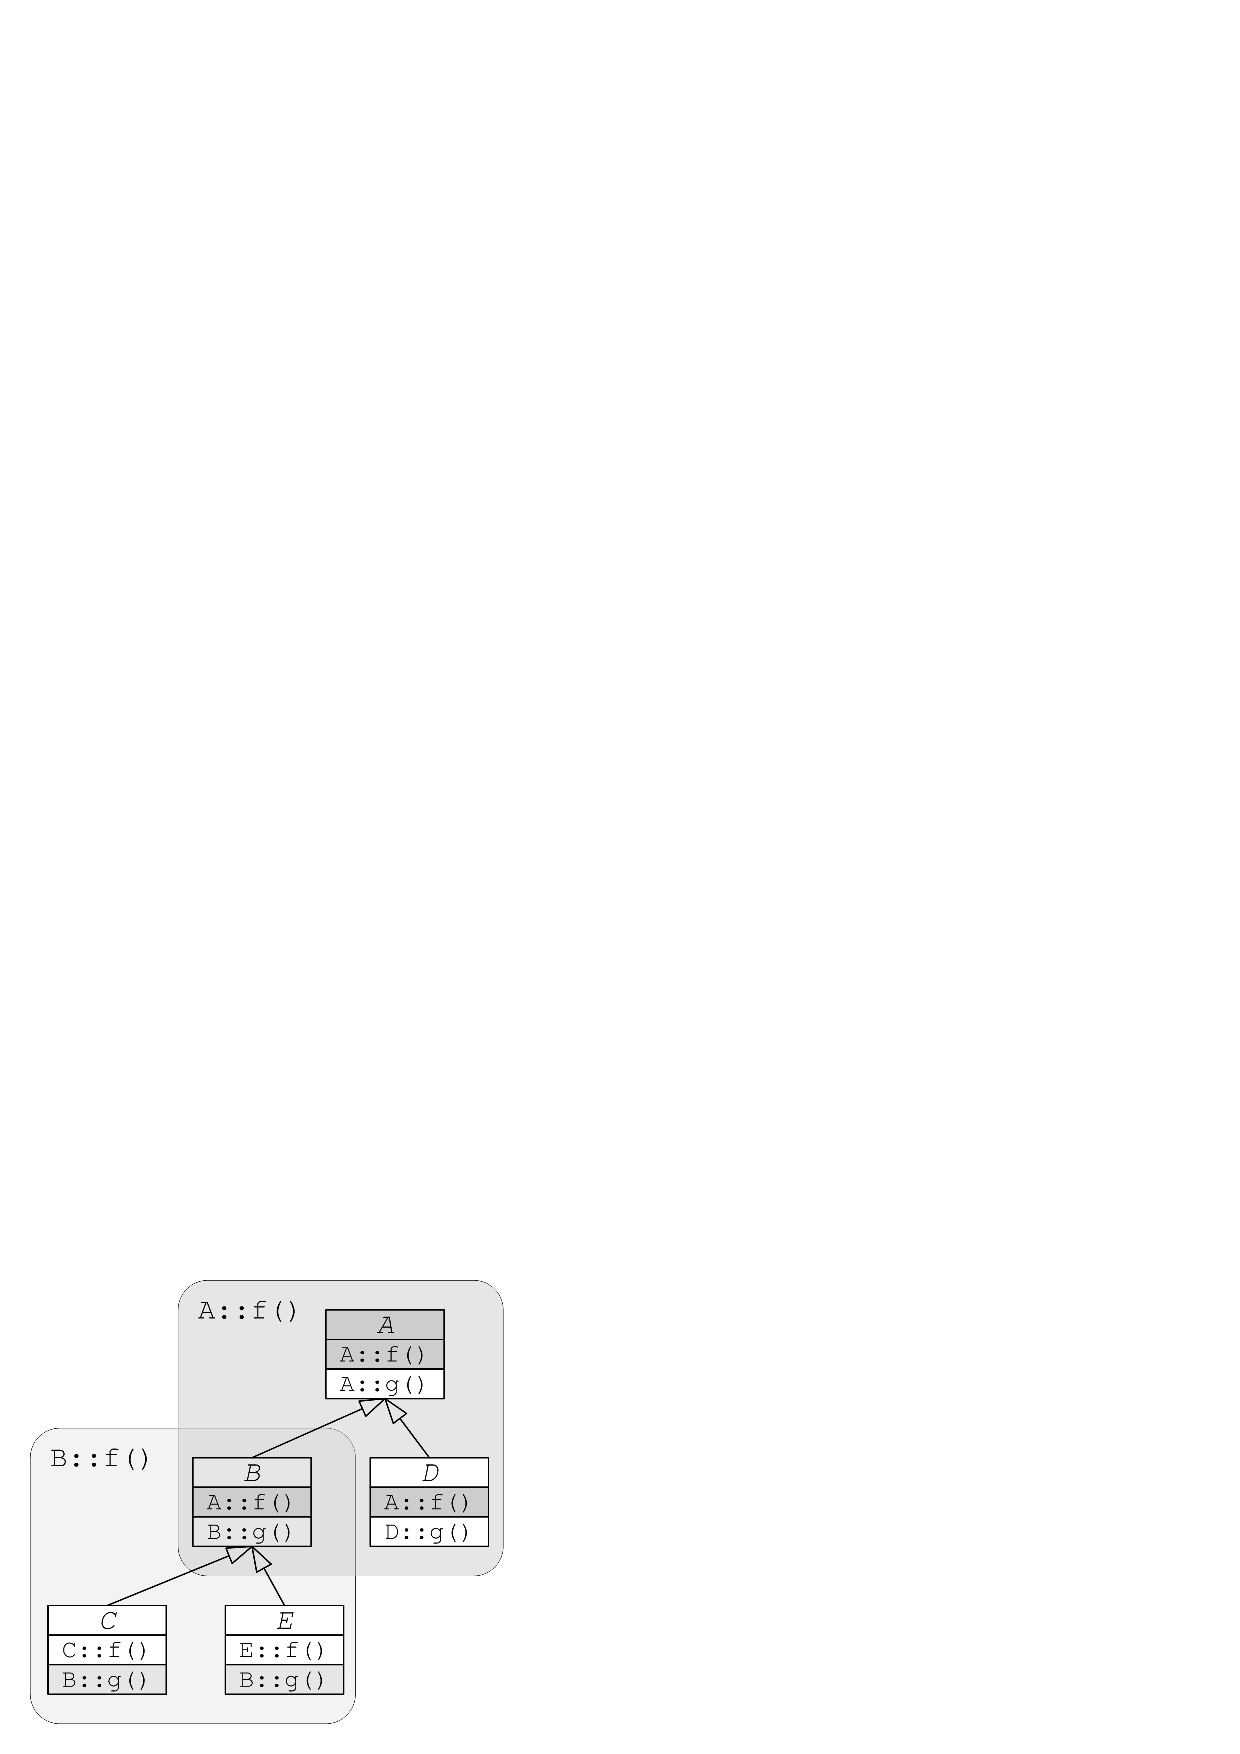
\includegraphics[scale=1.0]{images/fset.png}
\caption{Пример применения утверждения \ref{stmt:fsets_2} к иерархии наследования.}
\label{fig:fsets}
\end{figure}

\begin{figure}[htb!]
\hspace{2cm}
\begin{minipage}[b]{1cm}
\begin{cplusplus}
class A {
public:
    virtual void f() { /* .1. */ }
};

class B: public A {
public:
    virtual void f() { /* .2. */ }
};

class C: public B {
public:
    virtual void f() { A::f(); }
};
\end{cplusplus}
\end{minipage}
\caption{Пример иерархии наследования, для которой дополнительное требование утверждения \ref{stmt:fsets_2} может быть существенным.}
\label{listing:fset_failure}
\end{figure}

\begin{figure}[htb!]
\centering
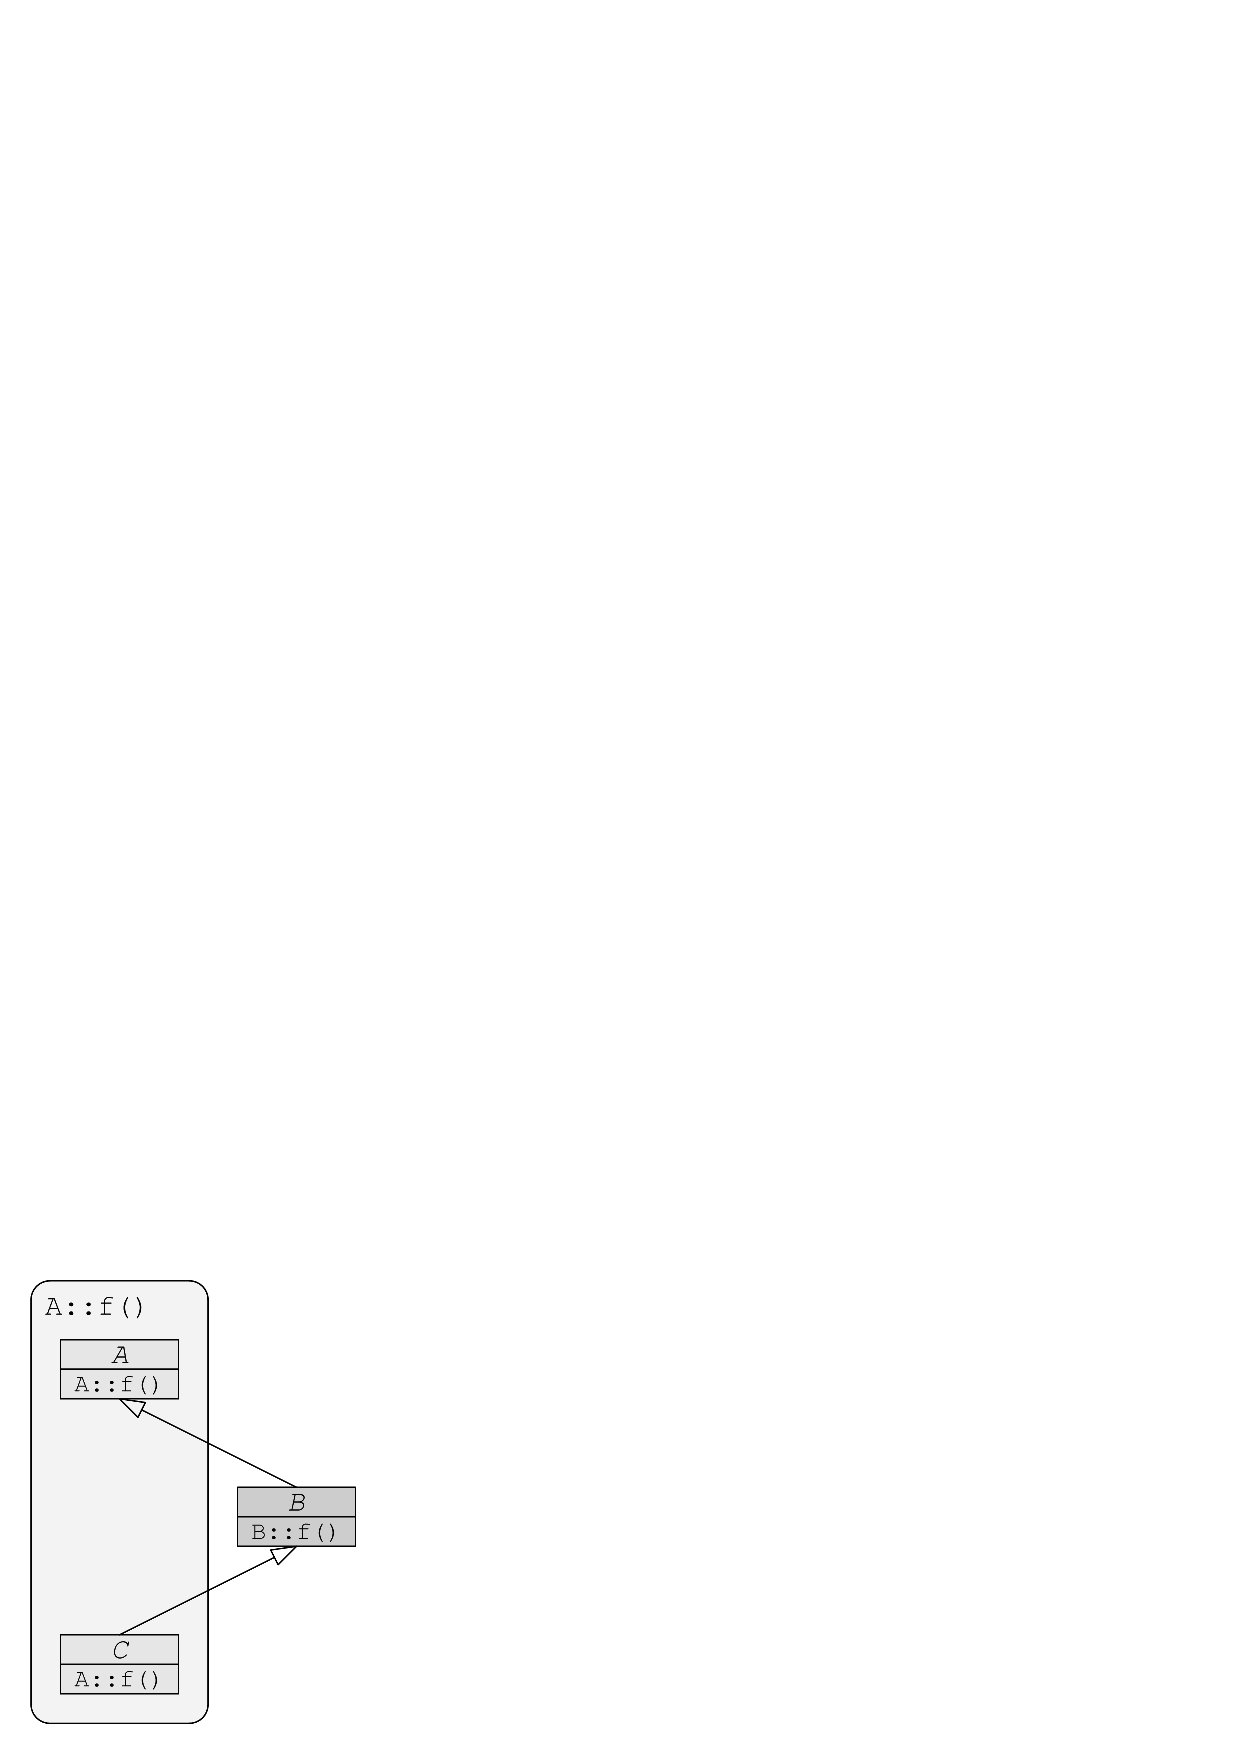
\includegraphics[scale=1.0]{images/fset_failure.png}
\caption{Пример иерархии наследования, для которой дополнительное требование утверждения \ref{stmt:fsets_2} существенно.}
\label{fig:fset_failure}
\end{figure}

На рисунке \ref{fig:fsets} приведен пример применения утверждения \ref{stmt:fsets_2} --- все классы из множества $\{\text{\lstinline{A}}, \text{\lstinline{B}}, \text{\lstinline{D}}\}$ имеют функцию \text{\lstinline{A::f}} на первой позиции в таблице виртуальных функций, и поэтому сужение иерархии наследования на множество $\{\text{\lstinline{A}}, \text{\lstinline{B}}, \text{\lstinline{D}}\}$ является деревом. Утверждение \ref{stmt:fsets_2} справедливо и для множества классов $\{\text{\lstinline{B}}, \text{\lstinline{C}}, \text{\lstinline{E}}\}$, имеющих функцию \text{\lstinline{B::g}} на второй позиции в таблице виртуальных функций.

Утверждение \ref{stmt:fsets_2} опирается на то, что при компиляции не возникает ситуации, когда однажды перекрытая в базовом классе виртуальная функция появляется в таблице виртуальных функций производного класса. Пример такой ситуации представлен на рис. \ref{listing:fset_failure}. При включении оптимизаций компиляторы GCC и MSVC не генерируют тело для функции \lstinline{C::f}, а просто записывают указатель на функцию \lstinline{A::f} в соответствующем месте в таблице виртуальных функций класса \lstinline{C}. Рис. \ref{fig:fset_failure} иллюстрирует применение утверждения \ref{stmt:fsets_2} к иерархии классов, представленной на рис. \ref{listing:fset_failure}. Как видно, применение утверждения в данном случае породило бы ограничение, для которого не выполнено (\ref{eq:restriction}).

Если в утверждении \ref{stmt:fsets_2} не требовать отсутствия ситуаций, подобных изображенной на рис. \ref{listing:fset_failure}, то не для всех полученных с использованием этого утверждения ограничений будет выполнено (\ref{eq:restriction}). Однако так как ситуации, подобные изображенной на рис. \ref{listing:fset_failure}, встречаются достаточно редко, то ограничения, для которых не выполняется (\ref{eq:restriction}), можно в случае возникновения конфликтов обработать отдельно.



\subsubsection{Анализ параметров виртуальных функций}\label{chapter:param_analysis}
\begin{statement}\label{stmt:param_size}
Пусть $A, C \in \gCa: \exists \, i: VT^A_i \ne \pure \wedge VT^C_i \ne \pure \wedge |\params(VT^A_i)| \ne |\params(VT^C_i)|$. Тогда для ограничения $\cR_{\ref{stmt:param_size}}^{AC} = \neg (A \sim C)$ выполнено (\ref{eq:restriction}).
\end{statement}

Согласно правилам наследования Си++, виртуальная функция производного класса должна иметь тот же список параметров, что и перекрываемая ею виртуальная функция базового класса \cite{cpp03}.
%cpp[10.3:2]

Используя методы статического анализа типов можно улучшить точность ограничений, порождаемых приведенным выше утверждением, сравнивая также восстановленные типы параметров, а не только их размер. Однако это требует реализации статического анализа типов, и может привести к проблемам в случае, когда в исходной программе используются структуры данных \lstinline{union}, или оператор \lstinline{reinterpret_cast<>}.

Также проблемы могут возникнуть, если пытаться восстановить суммарный размер параметров, анализируя обращения к стеку. Рассмотрим две функции, представленные на рисунке \ref{listing:param_size}.

\begin{figure}[htb!]
\hspace{2cm}
\begin{minipage}[b]{1cm}
\begin{cplusplus}
int a(int p0, int p1) {
    return p0;
}

int b(int p0, int p1) {
    return p1;
}
\end{cplusplus}
\end{minipage}
\caption{Пример функций, для которых нельзя восстановить суммарный размер параметров путем анализа обращений к стеку.}
\label{listing:param_size}
\end{figure}

Так как в каждой из функций один из аргументов не используется, то независимо от порядка передачи параметров, одна из функций будет обращаться в стек по большему смещению относительно {\tt esp}, чем другая. То есть, даже вычислив максимальное смещение относительно {\tt esp}, по которому происходило обращение к стеку внутри функции, нельзя с уверенностью сказать, что аргументов с большим смещением нет.

Если используется соглашение о вызовах, в котором очисткой стека занимается вызываемая сторона, то суммарный размер параметров определяется по эпилогу функции. В компиляторе MSVC для виртуальных функций по умолчанию используется соглашение \lstinline{thiscall}, обладающее этим свойством. В компиляторе GCC по умолчанию используется стандартное соглашение о вызовах Си, в котором очисткой стека занимается вызывающая сторона, и поэтому для программ, скомпилированных компилятором GCC, такой метод в большинстве случаев неприменим. Также стоит отметить, что для функций, не имеющих аргументов, как при использовании соглашения о вызовах \lstinline{thiscall}, так и при использовании стандартного соглашения о вызовах Си, генерируется один и тот же эпилог. В случае же наличия аргументов эпилоги отличаются, и используемый тип соглашения о вызовах можно определить.

С учетом всего вышесказанного, будем считать суммарный размер параметров определенным только для функций, использующих соглашение о вызовах, в котором очисткой стека занимается вызываемая функция.

\if 0
Заметим также, что верно и более общее утверждение.

\begin{statement}\label{stmt:param_size_2}
Пусть $A, C \in \gCa: \exists \, i: VT^A_i \ne \pure \wedge VT^C_i \ne \pure \wedge |\params(VT^A_i)| \ne |\params(VT^C_i)|$. Тогда для ограничения:
\begin{equation*}
\cR_{\ref{stmt:param_size_2}}^{AC} = \neg (A \sim^+ C) \vee \forall B \in \gCa: B \lhd A \wedge B \lhd C \Rightarrow |VT^B| < i
\end{equation*}
выполнено (\ref{eq:restriction}).
%\begin{equation*}
%\begin{aligned}
%&\neg (\Map(A) \sim^+ \Map(C)) \vee \\
%&\forall B \in \gCa: \Map(B) = \text{\lstinline{void}~} \vee \\
%&\quad (\Map(B) \lhd \Map(A) \wedge \Map(B) \lhd \Map(C) \Rightarrow |VT^B| < i)
%\end{aligned}
%\end{equation*}
\end{statement}

Действительно, если $i$-е функции в таблицах виртуальных функций классов $A$ и $C$ имеют различные размеры параметров, то это означает, что либо $A$ и $C$ не связаны наследованием и не имеют общих предков, либо для всех их общих предков $i$-я виртуальная функция не определена.
\fi



\subsubsection{Анализ вызовов виртуальных функций}\label{chapter:vcalls}
\begin{statement}\label{stmt:vcall}
Пусть $B, D \in \gCa: \exists \, i, j: VT_D^i \enspace \executes \enspace \text{\lstinline{this->}}VT_B^j\text{\lstinline{(...)}} \wedge VT_D^j \ne VT_B^j$. Тогда если в программе $P$ для приведения типов, не связанных наследованием, не используется преобразование \lstinline{reinterpret_cast<>}, или подобное ему, то для ограничения $\cR_{\ref{stmt:vcall}}^{BD} = B \lhd D$ выполнено (\ref{eq:restriction}).
\end{statement}

Если метод $m_D$ класса $D$ вызывает метод $m_B$ класса $B$ для того же объекта, для которого он был вызван сам (то есть для \lstinline{this}), то $m_B$ должен быть определен либо в самом классе $D$, либо в одном из его предков. Конечно, возможен также вариант с использованием оператора \lstinline{reinterpret_cast<>} --- например, $m_D$ может вызывать метод $m_B$ следующим образом: \lstinline{reinterpret_cast<}$B$\lstinline{*>(this)->}$m_B$, однако такие конструкции зачастую лишены смысла и в реальном коде встречаются редко. Поэтому аналогично с утверждением \ref{stmt:fsets_2}, требование отсутствия в программе $\bP$ приведения типов, не связанных наследованием, с использованием преобразования \lstinline{reinterpret_cast<>}, или подобного ему, можно опустить, и в случае возникновения конфликтов обработать отдельно ограничения, для которых не выполняется (\ref{eq:restriction}).

Если $m_B$ является виртуальной функцией, перекрытой в классе $D$, то остается только один вариант --- $B$ является предком $D$. При этом подразумевается, что при вызове виртуальной функции $m_B$ используется {\it статическое связывание}, потому как лишь в этом случае на этапе статического анализа известно, какая функция будет вызвана.

Для того, чтобы определить, действительно ли происходит вызов функции $VT_B^j$ для текущего объекта, необходимо знать способ передачи указателя \lstinline{this} в функции $VT_D^i$ и $VT_B^j$. Зная способ передачи указателя \lstinline{this} в функцию $VT_D^i$, можно провести анализ потока данных и для каждой инструкции в теле функции определить множество регистров и локаций памяти, в которых хранятся копии указателя \lstinline{this}. Используя построенные множества, и зная способ передачи указателя \lstinline{this} в функцию $VT_B^j$, можно определить, действительно ли она вызывается для текущего объекта.

Способ передачи указателя \lstinline{this} зависит от используемого функцией соглашения о вызовах. Используемые компиляторами GCC и MSVC соглашения о вызовах описаны в таблице \ref{fig:calling_conv}. По умолчанию и компилятор GCC, и компилятор MSVC используют соглашение о вызовах \lstinline{thiscall}.

%!!! перенести в обзор?

\begin{figure}[htb!]
\begin{tabular}{| l | l | l |}
\hline
Соглашение о вызовах & Очистка стека & Передача указателя {\color{keywordcolor}\textbf{this}} \\
\hline
MSVC cdecl & \multirow{2}{*}{Вызывающая функция} & \multirow{2}{*}{Первый параметр в стеке} \\
GCC cdecl & & \\
\hline
MSVC fastcall & \multirow{2}{*}{Вызывающая функция} & \multirow{2}{*}{регистр {\tt ECX}} \\
GCC fastcall & & \\
\hline
MSVC stdcall & \multirow{2}{*}{Вызываемая функция} & \multirow{2}{*}{Первый параметр в стеке} \\
GCC stdcall & & \\
\hline
MSVC thiscall & Вызываемая функция & регистр {\tt ECX} \\
\hline
GCC thiscall & Вызывающая функция & Первый параметр в стеке \\
\hline
GCC regparm & & регистр {\tt EAX} \\
\hline
\end{tabular}
\caption{Соглашения о вызовах, используемые компиляторами GCC и MSVC.}
\label{fig:calling_conv}
\end{figure}

Из таблицы \ref{fig:calling_conv} видно, что определение используемого функцией соглашения о вызовах по ее телу представляет некоторые сложности. Конечно, можно считать, что используется соглашение о вызовах \lstinline{thiscall}, что в большинстве случаев является правдой, однако такое предположение верно не всегда, и это может привести к неверным результатам. Однозначно выявить можно только использование соглашения о вызовах \lstinline{stdcall}, которое определяется по эпилогу функции. Однако на практике соглашение о вызовах \lstinline{stdcall} в программах на Си++ используется довольно редко.

В случае использования компилятора MSVC, виртуальной функции в регистре {\tt ECX} нельзя передать ничего кроме указателя \lstinline{this}, и поэтому если внутри функции происходит косвенное обращение к памяти с использованием значения, переданного в регистре {\tt ECX}, то это означает, что в {\tt ECX} был передан указатель \lstinline{this}. Так как компилятор MSVC по умолчанию использует соглашение о вызовах \lstinline{thiscall}, передающее указатель \lstinline{this} в регистре {\tt ECX}, то во многих случаях используемый способ передачи указателя \lstinline{this} можно определить.

Будем применять утверждение \ref{stmt:vcall} только в случаях, когда для функций $VT_D^i$ и $VT_B^j$, с использованием приведенных выше соображений, был восстановлен способ передачи указателя \lstinline{this}.




\subsubsection{Анализ виртуальных деструкторов}\label{chapter:destructors}
Сначала рассмотрим, какие действия должен производить деструктор:

\begin{itemize}
%% \renewcommand{\labelenumii}{(\alph{enumii})}
\item Выполнить заданный программистом в теле деструктора код.
\item Вызвать деструкторы для всех неунаследованных полей.
\item Вызвать деструкторы для всех базовых классов. При вызове деструктора какого-либо базового класса должен использоваться указатель на таблицу виртуальных функций этого класса. Это означает, что в деструкторе указатель на таблицу виртуальных функций будет несколько раз перезаписываться разными значениями, соответствующими различным базовым классам, как это представлено на рис. \ref{listing:destructor}.
\end{itemize}

То есть реальный деструктор --- это функция, сгенерированная компилятором, и написанный программистом код тела деструктора является лишь ее частью.

\begin{figure}[htb!]
\hspace{2cm}
\begin{minipage}[t]{0.1\textwidth}
\vspace{0pt}
\raggedleft
\includegraphics[scale=0.8]{images/destructor.png}
\end{minipage}
\hspace{0.5cm}
\begin{minipage}[t]{0.4\textwidth}
\vspace{0pt}
\raggedright
\begin{cplusplus}[emph={D}, emphstyle=\color{red}, emph={[2]B}, emphstyle={[2]\color{mygreen}}]
D::`destructor'() {
  this->`vfptr' = &D::`vftable';
  this->~D();

  /* ... */

  this->`vfptr' = &B::`vftable';
  this->~B();
}
\end{cplusplus}
\end{minipage}
\caption{Общая схема работы деструктора.}
\label{listing:destructor}
\end{figure}

При создании иерархий классов практически во всех случаях используется виртуальный деструктор --- он дает возможность единообразно уничтожать созданные объекты, при этом не беспокоясь о совместимости существующего кода с новыми классами, которые возможно будут добавлены в будущем. Более того, компилятор GCC даже выдает предупреждение в случае отсутствия виртуального деструктора в полиморфном базовом классе. При использовании виртуального деструктора объекты иерархии обычно создаются с помощью оператора \lstinline{new}, и уничтожаются с использованием оператора \lstinline{delete}. Но использование оператора \lstinline{delete} несет в себе некоторые проблемы. Рассмотрим пример, представленный на рис. \ref{listing:operator_delete}.

\begin{figure}[htb!]
\hspace{2cm}
\begin{minipage}[b]{1cm}
\begin{cplusplus}
struct V {
    virtual ~V();
};

struct W: V {
    void operator delete(void*);
};
\end{cplusplus}
\end{minipage}
\caption{Пример переопределения оператора \lstinline{delete} для класса с виртуальным деструктором.}
\label{listing:operator_delete}
\end{figure}

% [12.4:11]
Согласно правилам Си++ \cite{cpp03}, при вызове оператора \lstinline{delete} для объекта класса \lstinline{V} память должна быть освобождена с помощью глобального оператора \lstinline{::operator delete(void*)}, в то время как для объекта класса \lstinline{W} должен использоваться \lstinline{W::operator delete(void*)}. Так как в месте вызова виртуального деструктора фактический класс уничтожаемого объекта неизвестен, то невозможно определить, какой оператор \lstinline{delete} необходимо вызывать. Поэтому как компилятор GCC, так и компилятор MSVC вместо указателя на деструктор хранят в таблице виртуальных функций указатель на так называемый <<освобождающий деструктор>>\footnote{англ. deleting destructor.}, который в случае необходимости освобождает память с помощью соответствующего оператора \lstinline{delete}.

И в компиляторе GCC, и в компиляторе MSVC код освобождающего деструктора имеет вполне определенную структуру, и может быть идентифицирован с помощью сравнения сигнатур. Теперь, когда место освобождающего деструктора в таблице виртуальных функций определено, можно сформулировать следующее утверждение:

\begin{statement}\label{stmt:destructors}\label{stmt:last_good}
Пусть $B, D \in \gCa: D \text{\lstinline{::~}} \! D \enspace \executes \enspace \text{\lstinline{this->`vfptr'}}\text{~\lstinline{= &}}VT_B$, где поле \lstinline{`vfptr'} хранит указатель на таблицу виртуальных функций. Тогда для ограничения $\cR_{\ref{stmt:destructors}}^{BD} = B \lhd D$ выполнено (\ref{eq:restriction}).
\end{statement}

Казалось бы, это утверждение будет выполнено для всех классов, являющихся предками $D$, однако из-за примененных компилятором оптимизаций это может оказаться не так. Эксперименты с компиляторами GCC и MSVC показали, что в случае использования пустых деструкторов в результате оптимизаций компилятор удаляет последовательные перезаписи поля \lstinline{this->`vfptr'}, оставляя лишь последнюю. Так как в последнюю очередь всегда вызывается деструктор базового класса всей иерархии, то как минимум для него утверждение будет выполнено. Если же у $D$ нет базовых классов, то перезапись поля \lstinline{this->`vfptr'} будет произведена только один раз --- указателем на $VT_D$.

Для того, чтобы определить, действительно ли происходит присваивание вида \lstinline{this->`vfptr'}\lstinline{ = &}$VT_B$, необходимо знать способ передачи указателя \lstinline{this} освобождающему деструктору, и провести анализ потока данных. Как было сказано в главе \ref{chapter:vcalls}, способ передачи указателя \lstinline{this} зависит от используемого освобождающим деструктором соглашения о вызовах.

В компиляторе MSVC, независимо от установленного соглашения о вызовах по умолчанию, для освобождающего деструктора всегда используется соглашение о вызовах \lstinline{thiscall}. В компиляторе GCC используемое для освобождающих деструкторов соглашение о вызовах зависит от установленных по умолчанию атрибутов функций. Так как параметры и структура освобождающего деструктора известны, и различных соглашений о вызовах, используемых компилятором GCC, не так много (см. главу \ref{chapter:vcalls}), то используемое соглашение о вызовах можно определить на этапе сравнения сигнатур.





\subsubsection{Ненадежные источники информации}\label{chapter:unreliable}
Отличительная особенность ограничений, получаемых с использованием описанных выше утверждений --- это их <<надежность>>. Даже при ослабленных требованиях, для большинства встречающихся на практике программных продуктов вероятность получить с их использованием ограничения, для которых не выполнено (\ref{eq:restriction}), близка к нулю. Но существуют и другие источники информации, которые дают ограничения, для которых (\ref{eq:restriction}) не выполняется лишь в небольшом проценте случаев. Приведем несколько примеров таких источников информации.

Пусть $\textit{MaxThisAccessOffset}_A$ --- максимальное смещение относительно указателя \lstinline{this}, по которому происходит обращение к памяти в виртуальных функциях класса $A$, а также в функциях, вызываемых из виртуальных. Пусть $B, D \in \gCa: \textit{MaxThisAccessOffset}_B < \textit{MaxThisAccessOffset}_D$. Тогда для ограничения $\cR_?^{BD} = B < D$ с большой вероятностью выполнено (\ref{eq:restriction}).

Действительно, при наследовании в большинстве случаев добавляется дополнительная функциональность, и для реализации этой функциональности зачастую требуется хранение некоторой дополнительной информации. Эта дополнительная информация добавляется к классу в форме полей, которые затем используются в виртуальных функциях. Из того факта, что добавленные в производном классе поля всегда имеют большее смещение, чем унаследованные \cite{gray94, gccabi}, напрямую следует приведенное выше соображение. Однако в силу того, что для встречающихся на практике программ это соображение не всегда выполнено, его нельзя напрямую использовать для восстановления отношения $<$.

Еще одним примером ненадежного источника информации может служить утверждение \ref{stmt:vcall}, применяемое не только к функциям, для которых используемый метод передачи указателя \lstinline{this} может быть однозначно восстановлен, но и для всех остальных в предположении, что используется соглашение о вызовах по умолчанию.




























